\documentclass[border=1cm]{standalone}
%\documentclass{article}
\usepackage{tikz}
\usepackage[width=0.5,tiewidth=0.7]{strands}

\begin{document}
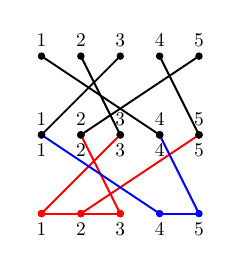
\begin{tikzpicture}[scale=1,text=black]
%\permutation[tkzpic=0]{4,3,1,5,2}
\vpartition[
bullb=0,
floor=0,
tkzpic=0,
type=2
]{{5}}
\tie[color=red,bull=1,bulletie=0.04,style=solid,tieheight=0]{{1},{2},{3}}
\tie[color=red,bull=1,bulletie=0.04,style=solid]{{3,1},{1,0}}
\tie[color=red,bull=1,bulletie=0.04,style=solid]{{5,1},{2,0}}
\tie[color=red,bull=1,bulletie=0.04,style=solid]{{2,1},{3,0}}
\tie[color=blue,bull=1,bulletie=0.04,style=solid]{{1,1},{4,0},{5,0},{4,1}}
 {[color=green]\permutation[tkzpic=0,floor=1]{4,3,1,5,2}};

\end{tikzpicture}
 \strands[height=0.2,bendbraid=20,type=2]{s1*s2*s1*s4*s3*s2}
 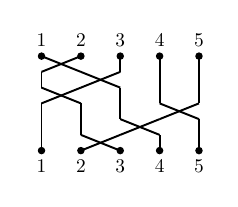
\begin{tikzpicture}
 \permutation[
 height=0.2,
 bullb=0,
 floor=5,
 tkzpic=0,
 type=1
 ]{2,1,3,4,5}
 \permutation[
 height=0.2,
 bulla=0,
 bullb=0,
 floor=4,
 tkzpic=0,
 type=0
 ]{1,3,2,4,5}
 \permutation[
 height=0.2,
 bulla=0,
 bullb=0,
 floor=3,
 tkzpic=0,
 type=0
 ]{2,1,3,4,5}
  \permutation[
  height=0.2,
  bulla=0,
  bullb=0,
  floor=2,
  tkzpic=0,
  type=0
  ]{1,2,3,5,4}
 \permutation[
 height=0.2,
 bulla=0,
 bullb=0,
 floor=1,
 tkzpic=0,
 type=0
 ]{1,2,4,3,5}
 \permutation[
 height=0.2,
 bulla=0,
 floor=0,
 tkzpic=0,
 type=-1
 ]{1,3,2,4,5}
 \end{tikzpicture}
 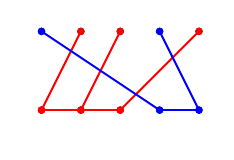
\begin{tikzpicture}
 \vpartition[
 floor=0,
 tkzpic=0,
 type=0
 ]{{5}}
 \tie[color=red,bull=1,bulletie=0.04,style=solid,tieheight=0]{{1},{2},{3}}
 \tie[color=red,bull=1,bulletie=0.04,style=solid]{{2,1},{1,0}}
 \tie[color=red,bull=1,bulletie=0.04,style=solid]{{3,1},{2,0}}
 \tie[color=red,bull=1,bulletie=0.04,style=solid]{{5,1},{3,0}}
 \tie[color=blue,bull=1,bulletie=0.04,style=solid]{{1,1},{4,0},{5,0},{4,1}}
 
 \end{tikzpicture}
\end{document}